% !TeX encoding = UTF-8
% !TeX spellcheck = en_US
\documentclass{article}
\usepackage[nostamp]{../moodle}
\ifxetex % FOR XELATEX
	\usepackage{fontspec}
\else %% FOR PDFLATEX
	\usepackage[utf8]{inputenc} % necessary
	\usepackage[T1]{fontenc} % necessary
\fi
\usepackage{circuitikz}
\begin{document}

\section*{Introduction}

This document is intended to check the support of circuitikz.

\begin{quiz}{Circuitikz}

\begin{multi}{Multi}
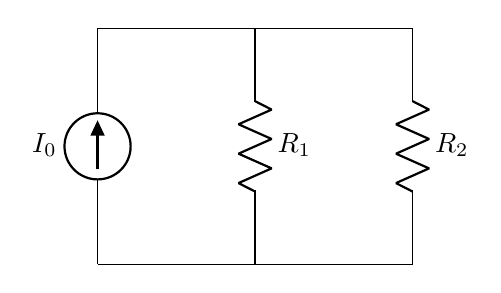
\begin{tikzpicture}[american]
\draw (0,0) to[isource, l=$I_0$] (0,3) --(2,3) to[R=$R_1$] (2,0) -- (0,0);
\draw (2,3) -- (4,3) to[R=$R_2$] (4,0) -- (2,0);
\end{tikzpicture}
\item[feedback={}]* 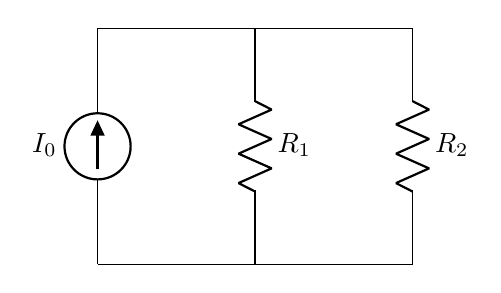
\begin{tikzpicture}[american]
\draw (0,0) to[isource, l=$I_0$] (0,3) --(2,3) to[R=$R_1$] (2,0) -- (0,0);
\draw (2,3) -- (4,3) to[R=$R_2$] (4,0) -- (2,0);
\end{tikzpicture}
\item[feedback={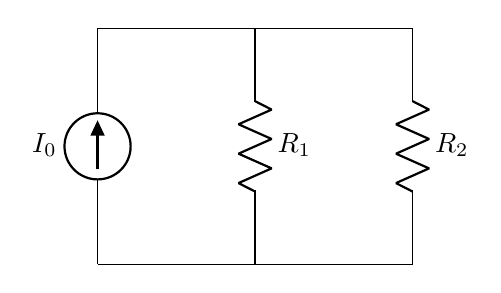
\begin{tikzpicture}[american]
\draw (0,0) to[isource, l=$I_0$] (0,3) --(2,3) to[R=$R_1$] (2,0) -- (0,0);
\draw (2,3) -- (4,3) to[R=$R_2$] (4,0) -- (2,0);
\end{tikzpicture}}] toast
\end{multi}

\end{quiz}

\end{document}
